\chapter{Progettazione concettuale}
    \section{Class Diagram del dominio del problema}

    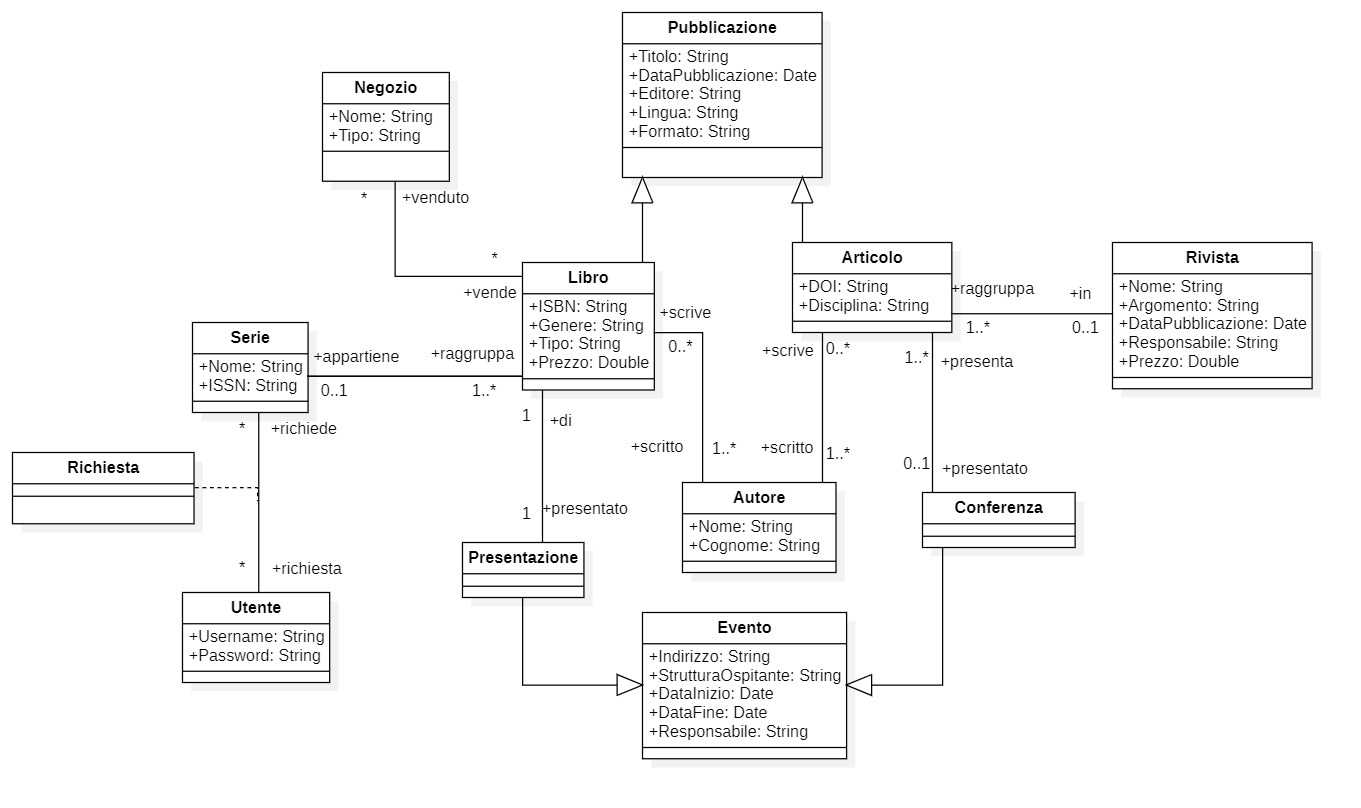
\includegraphics[scale=0.25, center]{Immagini/CD_dominio_del_problema.png}
        
        \newpage

    \section{Dizionario delle classi}

    \begin{longtable}[c]{|l|l|}
      \hline
      \textbf{Classe} &
        \textbf{Attributi} \\ \hline
      \endfirsthead
      %
      \endhead
      %
      Articolo &
        \begin{tabular}[c]{@{}l@{}}Eredita da Pubblicazione, abbiamo inoltre:\\ DOI (String): Identificativo di un oggetto\\ digitale.\\ Disciplina (String): Disciplina approfondita\\ dall'articolo.\end{tabular} \\ \hline
      Autore &
        \begin{tabular}[c]{@{}l@{}}Nome (String): Nome di un autore.\\ Cognome (String): Cognome di un autore.\end{tabular} \\ \hline
      Conferenza &
        Ereditati da Evento. \\ \hline
      Evento &
        \begin{tabular}[c]{@{}l@{}}Indirizzo (String): Indirizzo a cui è associato\\ un evento.\\ StrutturaOspitante (String): Struttura che\\ ospita un evento.\\ DataInizio (Date): Data in cui un certo\\ evento ha inizio.\\ DataFine (Date): Data in cui un certo evento\\ ha fine.\\ Responsabile (String): Nome e cognome\\ del responsabile di un evento.\end{tabular} \\ \hline
      Libro &
        \begin{tabular}[c]{@{}l@{}}Eredita da Pubblicazione, abbiamo inoltre:\\ ISBN (String): Identificativo di un libro.\\ Tipo (String): Tipo di un libro (Didattico o \\ Romanzo)\\ Prezzo (Double): Prezzo di un libro.\end{tabular} \\ \hline
      Negozio &
        \begin{tabular}[c]{@{}l@{}}Nome (String): Nome di un negozio.\\ Tipo (String): Tipo di un negozio (Online o\\ Fisico).\end{tabular} \\ \hline
      Presentazione &
        Ereditati da Evento. \\ \hline
      Pubblicazione &
        \begin{tabular}[c]{@{}l@{}}Titolo (String): Titolo di un libro o un\\ articolo scientifico.\\ DataPubblicazione (Date): Data di\\ uscita di una pubblicazione.\\ Editore (String): Casa editrice di una\\ pubblicazione.\\ Lingua (String): Lingua in cui è scritta una\\ pubblicazione\\ Formato (String): Formato di una \\ pubblicazione (Cartaceo, Digitale o \\ Audiolibro).\end{tabular} \\ \hline
      Rivista &
        \begin{tabular}[c]{@{}l@{}}Nome (String): Nome di una rivista \\ scientifica.\\ Argomento (String): Argomento di cui si\\ occupa la rivista.\\ DataPubblicazione (Date): Data in cui è \\ stata pubblicata una rivista scientifica.\\ Responsabile (String): Nome e cognome \\ del responsabile della rivista.\\ Prezzo (Double): Prezzo di una rivista\\ scientifica.\end{tabular} \\ \hline
      Serie &
        \begin{tabular}[c]{@{}l@{}}Nome (String): Nome di una serie di libri.\\ ISSN (String): Identificativo di una serie.\end{tabular} \\ \hline
      Utente &
        \begin{tabular}[c]{@{}l@{}}Username (String): Nome utente di un\\ account.\\ Password (String): Password di un account.\end{tabular} \\ \hline
      \end{longtable}
        
    \section{Dizionario delle associazioni}